\documentclass[12pt,a4paper]{article}
\usepackage[utf8]{inputenc}
\usepackage[russian]{babel}
\usepackage[width=17cm,top=1cm,height=27cm]{geometry}
\usepackage{graphicx}
\title{Численные методы(Мусаева)}

\date{May 2019}

\begin{document}
\begin{titlepage}
\begin{center}
2019 год
\vspace {8cm}



{ \LARGEПрактикум по численным методам:\\ методы поиска корней уравнения $f(x)=0$}\\
\vspace {8cm}
\bigskip Мусаева Аида, группа 208
\end{center}
\vfill


\vfill

\end{titlepage}

\section{Метод деления пополам (метод бисекций)}

\text{Задана функция $f(x) = x^3-3x-2e^{-x}$ и требуется найти корень уравнения $f(x)=0$. Для этого необходимо найти такой отрезок $[a, b]$, что $f(a)*f(b) < 0$. Тогда по теореме Больцано-Коши внутри отрезка $[a,b]$ существует точка $c$, в которой значение функции равно 0.
\\ \\
Итерационный метод бисекций состоит в построении последовательности вложенных отрезков ${[a_n, b_n] \in [a_n-1, b_n-1] ⊂ … ⊂ [a, b]},$ на концах которых функция принимает значения разных знаков. Каждый последующий отрезок получают делением пополам предыдущего. На каждом шаге итерации мы вычисляем значение $\xi= (a_n+b_n) / 2$ и значение функции $f(\xi)$ в этой точке. После проверяем, является ли корнем нашего уравнения и в противном случае добавляем в последовательность отрезков один из отрезков $[a_n,\xi]$ или $[a_n,\xi]$ на концах, которого функция имеет разные знаки.

Искомый отрезок определяется графически. Корень лежит на отрезке [0, 1].

График:}\\

\begin{figure}[h]
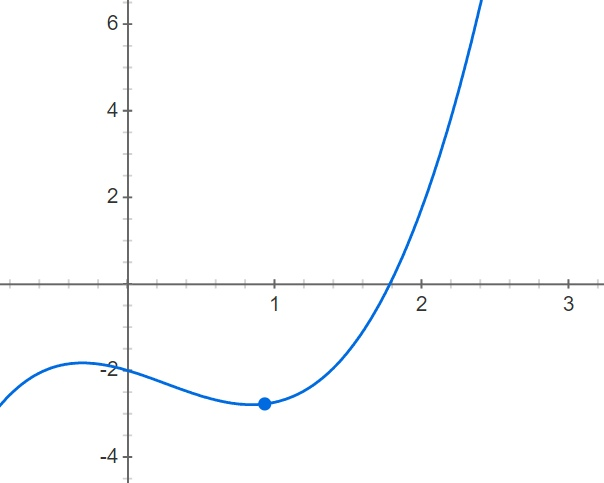
\includegraphics[width=\linewidth]{pic.jpg}
\caption{}
\label{fig:}
\end{figure}

\subsection{Код программы}
\begin{verbatim}
#include "stdafx.h"
#include <iostream>
#include "math.h"
#include <cmath>
using namespace std;

double f(double x) {
	/*return sin(pow(x, 2)) - 6 * x + 1;*/
	return pow(x,3)-3*x-2*exp(-x);
}

int main()
{
	const double eps = pow(10, -6);
	double an = 1;
	double bn = 2;
	int k = 0;
	double x0;

	while (fabs(an - bn) > 2 * eps) {
		x0 = (an + bn) / 2;
		if (f(x0) == 0)
			break;
		k++;
		if (f(x0)*f(an) < 0)
			bn = x0;
		else
			an = x0;
	}
	cout << x0 << endl << k;
	return 0;

}
\end{verbatim}
\subsection{Результат выполнения программы}
\text{Корень $x \approx 1.78$, 19 итераций.}\\
\section{Метод простых итераций}
\text{Этот метод заключается в замене исходного уравнения эквивалентным ему уравнением $x=\phi(x)$. Тогда последовательность $x_{n+1} = \phi(x_n)$ будет при $n \to \infty$ она будет сходиться к корню уравнения $f(x)=0$.\\\\
Функция: $f(x) = arctan(x)-ln(x)$
}\\\\
\vspace {8cm}
\begin{figure}[h]
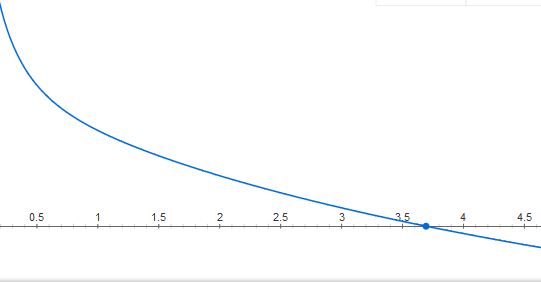
\includegraphics[width=\linewidth]{pic2.PNG}
\caption{}
\label{fig:}
\end{figure}

\subsection{Код программы}
\begin{verbatim}
import numpy as np

f = lambda x: np.arctan(x)-np.log(x)
phi = lambda x: np.exp(np.arctan(x))

def Iteration(f, x0, eps):
    x = x0
    k = 0;
    while True:
        y = f(x)
        k+=1;
        if abs(y - x) < eps:
            return y, k
        else:
            x = y


res, i = Iteration(phi, 3, 1e-6)
print(res)
print(i)
\end{verbatim}
\subsection{Результат выполнения программы}\\
\text{
Корень $x \approx 3.6925854568405736$, 11 итераций.\\}
\section{Метод Ньютона}
\text{Метод состоит в построении итерационной последовательности $x_n+1 = x_n - f(x_n)/f'(x_n)$, которая сходится к корню уравнения $f(x) = 0$, если функция $f(x)$ определена и дважды дифференцируема на $[a, b]$.}
\subsection{Код программы}
\begin{verbatim}
#include "stdafx.h"
#include <iostream>
#include <math.h>

using namespace std;

double f(double x){
	return pow(x,3)-3*x-2*exp(-x);
}

double df(double x){
	return 3*pow(x,2)+2*exp(-x);
}

int main()

{
	const double eps = pow(10, -6);
	int k = 0;
	double x = 0.5;
	double y = f(x);
	double dy = df(x);
	double xn = x - y / dy;
	while (abs(xn - x) > eps){

		k++;
		x = xn;
		y = f(x);
		dy = df(x);
		xn = x - y / dy;
	}

	cout << xn << endl <<  k << endl;

	return 0;
}
\end{verbatim}
\subsection{Результат выполнения программы}\\
\text{Корень $x \approx 1.785$, 10 итераций.}\\
\end{document}